% Harrison Zafrin / Collin Chudwick
% MIR - Final Paper
%----------------------------------------------------------------------------------------
% PACKAGES AND OTHER DOCUMENT CONFIGURATIONS
%----------------------------------------------------------------------------------------

\documentclass{article}
\usepackage{icmc2015template}
\usepackage{times}
\usepackage{ifpdf}
\usepackage{soul}
\usepackage[english]{babel}
\usepackage{cite}
\usepackage{subcaption}
\usepackage{caption}
\usepackage{graphicx}% http://ctan.org/pkg/graphicx
\usepackage{epsfig}
\usepackage{float}
\usepackage{multirow}

%%%%%%%%%%%%%%%%%%%%%%% Some useful packages %%%%%%%%%%%%%%%%%%%%%%%%%%%%%%%
%%%%%%%%%%%%%%%%%%%%%%% See related documentation %%%%%%%%%%%%%%%%%%%%%%%%%%
\usepackage{amsmath} % popular packages from Am. Math. Soc. Please use the 
\usepackage{amssymb} % related math environments (split, subequation, cases,
\usepackage{amsfonts}% multline, etc.)
\usepackage{bm}      % Bold Math package, defines the command \bf{}
%\usepackage{paralist}% extended list environments
%%subfig.sty is the modern replacement for subfigure.sty. However, subfig.sty 
%%requires and automatically loads caption.sty which overrides class handling 
%%of captions. To prevent this problem, preload caption.sty with caption=false 
%\usepackage[caption=false]{caption}
%\usepackage[font=footnotesize]{subfig}

% ====================================================
% ================ Define title and author names here ===============
% ====================================================
%user defined variables
\def\papertitle{Autonomous Multi-Track Mixing Using Multiple Linear Regression}
\def\firstauthor{Harrison Zafrin}
\def\secondauthor{Collin Chudwick}
\def\thirdauthor{Third Author}
\def\fourthauthor{Fourth Author}
\def\fifthauthor{Fifth Author}
\def\sixthauthor{Sixth Author}

% adds the automatic
% Saves a lot of ouptut space in PDF... after conversion with the distiller
% Delete if you cannot get PS fonts working on your system.

% pdf-tex settings: detect automatically if run by latex or pdflatex
\newif\ifpdf
\ifx\pdfoutput\relax
\else
   \ifcase\pdfoutput
      \pdffalse
   \else
      \pdftrue
\fi

\ifpdf % compiling with pdflatex
  \usepackage[pdftex,
    pdftitle={\papertitle},
    pdfauthor={\firstauthor, \secondauthor, \thirdauthor},
    bookmarksnumbered, % use section numbers with bookmarks
    pdfstartview=XYZ % start with zoom=100% instead of full screen; 
                     % especially useful if working with a big screen :-)
   ]{hyperref}
  %\pdfcompresslevel=9

  \usepackage[pdftex]{graphicx}
  % declare the path(s) where your graphic files are and their extensions so 
  %you won't have to specify these with every instance of \includegraphics
  \graphicspath{{./figures/}}
  \DeclareGraphicsExtensions{.pdf,.jpeg,.png}

  \usepackage[figure,table]{hypcap}

\else % compiling with latex
  \usepackage[dvips,
    bookmarksnumbered, % use section numbers with bookmarks
    pdfstartview=XYZ % start with zoom=100% instead of full screen
  ]{hyperref}  % hyperrefs are active in the pdf file after conversion

  \usepackage[dvips]{epsfig,graphicx}
  % declare the path(s) where your graphic files are and their extensions so 
  %you won't have to specify these with every instance of \includegraphics
  \graphicspath{{./figures/}}
  \DeclareGraphicsExtensions{.eps}

  \usepackage[figure,table]{hypcap}
\fi

%setup the hyperref package - make the links black without a surrounding frame
\hypersetup{
    colorlinks,%
    citecolor=black,%
    filecolor=black,%
    linkcolor=black,%
    urlcolor=black
}


% ====================================================
% ================ Title and author info starts here ===============
% ====================================================
% Title.
% ------
\title{\papertitle}

% Authors
% Please note that submissions are anonymous, therefore 
% authors' names should not be VISIBLE in your paper submission.
% They should only be included in the camera-ready version of accepted papers.
% uncomment and use the appropriate section (1, 2 or 3 authors)
%
% Single address
% To use with only one author or several with the same address
% ---------------
\twoauthors
  {1.5in}
  {\firstauthor} {NYU Music Technology \\  %
    {\tt \href{mailto:hzz200@nyu.edu}{hzz200@nyu.edu}}}
  {\secondauthor} {NYU Music Technology \\  %
    {\tt \href{mailto:crc445@nyu.edu}{crc445@nyu.edu}}}

%----------------------------------------------------------------------------------------
% BEGIN DOCUMENT
%----------------------------------------------------------------------------------------
\begin{document}

\capstartfalse
\maketitle
\capstarttrue

%----------------------------------------------------------------------------------------
% ABSTRACT AND KEYWORDS
%----------------------------------------------------------------------------------------
\begin{abstract}
In this paper, an autonomous mixing system is implemented using machine learning to estimate and apply fader weighting coefficients.  While in previous research this algorithm was shown to be an effective form of autonomous mixing, the goal of this paper is to build upon the previous implementation by expanding the extracted feature set, and comparing the models efficiency across genre.  In this off-line MATLAB implementation, audio examples are provided to show the result of multiple linear regression as a prediction model, and its accuracy is calculated via the mean squared error between the ground truth and the predicted coefficients.  The current implementations validity is evaluated and future research directions are established. To download the code used to run this experiment, visit https://github.com/bombsandbottles/Automatic-Mixing-Using-Multiple-Linear-Regression.
\end{abstract}


%----------------------------------------------------------------------------------------
% INTRODUCTION
%----------------------------------------------------------------------------------------
\section{Introduction}
\label{sec:Introduction}

% Often the last stage of the songwriting/production process, mixing ensures that the final product is perceived in the fashion which it was intended.  A more textbook definition for mixing can be given as the combination of multiple audio signals, modifying them from an amplitude, spatial, and spectral level as a means of creating a cohesive whole.  As professional music producers and engineers, the authors understand the plight and struggle of pouring tens of hours into a mix down only to wind up being disappointed when hearing the final product compared against another song.  Mixing is also notoriously difficult, requiring years of experience, expert taste, and fine tuned hearing.  If the producer/artist can't mix the song to satisfaction, he/she is left with no other choice but to hire professional help.  The goal of this research is to eliminate this struggle, and shift the focus back to writing phenomenal music.

Among the stages involved in studio music production, the art of mixing plays a pivotal role between tracking and mastering.  Since it is the primary process that determines the balance of the final recording, it is an essential step that is often considered an artistic job done by a skilled and experienced engineer who is also trusted by the lead artists to follow the aesthetic of the song.  Due to this fact that record production is never complete without mixing, a difficult situation can easily arise for any artist who is preparing a demo recording of their own song but struggles with writing and recording in anticipation for the mixing phase.  Interestingly, the growth of digital music that has developed over the past couple decades and had a direct impact on the increased importance and skill required of mixing has simultaneously given an incredible amount of power to smaller-budget artists who can record, mix and master entirely on their personal computer.  

This situation has caused a specific problem in the record production industry: without the skills and experience of a professional audio mixer, artists may become distracted and ultimately hampered by the notion of a mixing phase that will be an essential part of their record.  This could lead to focus being taking away from the songwriting process or worse, artists being led to choices based on the results of poor mixes.  It is therefore the goal of this research to help eliminate the presented problem by providing artists with intelligent mixing tools.  These tools aim to allow artists to automatically create mixes of their recorded tracks that sound balanced and professional, thereby reducing the consideration required by artists for their mixes.  

As can be expected to those with experience in audio engineering, the mix down process can be thought of as a mathematical summation of $N$ total tracks with varying weight.  Currently there are three main models built to decide \textbf{how} an autonomous system deals with assigning those weighting coefficients.  The first are models built upon a cross adaptive approach, meaning the systems decisions are informed by other variables in the system \cite{mansbridge2012implementation}.  The second are known as knowledge engineered systems, which operate around a predefined set of rules based upon best mixing practices.  The best definition as to what defines ``best mixing practices''can be found in a comprehensive review of the audio engineering literature recently conducted by Pedro Pestana \cite{pestana2013automatic}.  These rules allow a dimension of semantic data to be incorporated into the model as opposed to relying solely on the extraction of low-level audio features.  The third model which is the focus of this paper revolves around machine learning, using training data as a means of informing future decisions.  Therefore, if the mix down is a quantifiable process, theoretically a system can be trained on professionally mixed tracks and match those idealized targets to raw data \cite{scott2011automatic}.

This experiment will specifically emulate and expand upon the work of Scott et al. \cite{scott2011automatic} by comparing estimated ground truth weighting coefficients computed through non-negative least squares minimization to predicted weighting coefficients computed through multiple linear regression.  Once weighting coefficients have been estimated, new mixes can be made that follow the coefficients in an attempt to compare the success of various variables, specifically through both listening tests and measures of the mean square error.  This approach allows for simple comparison between the values of certain features and their difference among two prominent genres: pop and rock.  Specifically, the pop genre will create training sets based on the following stems from top-40 pop female artists: Britney Spears - “Break The Ice”, Betty Who - “All Of You”, Britney Spears - “Gimme More”, Katy Perry - “E.T.”, Katy Perry - “California Gurls”, Oh Land - “Renaissance Girls”.  The resultant coefficients will be analyzed on the stems found in Lady Gaga - “Alejandro”.  Similarly, the rock genre will create training sets based on the following stems provided by MedleyDB and Bittner et al. \cite{bittner2014medleydb}: The Districts - “Vermont”, The Scarlet Brand - “Les Fleurs Du Mal”, Purling Hiss - “Lolita”, Meaxic - “You Listen”, Meaxic - “Take A Step”, Creepoid - “Old Tree”, The So So Glos - “Emergency”.  The resultant coefficients will be analyzed on the stems found in Big Troubles - “Phantom”. 
	
% The paper is broken up as follows: Section \ref{sec:Algorithm and Implementation} includes a discussion of the specific algorithms and implementation utilized in the research.  It specifically covers weight estimation in section \ref{subsec:Ground-Truth Weight Estimation}, feature extraction in section \ref{subsec:Feature Extraction}, multiple linear regression in section \ref{subsec:Multiple Linear Regression}, and finally top-down combination of these various elements in section \ref{subsec:Autonomously Mix} that produce the final results and accuracy of the algorithms used.  Section \ref{sec:Results} provides a detailed analysis of the experimental results, including a number of numerical and auditory displays for analysis of the algorithms success.  Finally, section \ref{sec:Conclusion} ends the paper by drawing relevant conclusions for automatic mixing based on our implementation and results, as well as providing direction for future study. 

%----------------------------------------------------------------------------------------
% ALGORITHM AND IMPLEMENTATION
%----------------------------------------------------------------------------------------
\section{Algorithm and Implementation}
\label{sec:Algorithm and Implementation}

In this section, the process on how to perform autonomous mixing with multiple linear regression is detailed.  In summation, the process can be broken down into the following steps: First, a ground truth weight estimation per stem is calculated using non-negative least squares (NNLS).  Once we have our ground truth weights, we collect both temporal and spectral audio features from our training set.  This model assumes that when these features are linearly combined, they are synonymous with fader coefficients in a multi-track system.  From here, a multiple linear regression is performed to predict weighting coefficients for the test data based upon the genre related training stems.  The predicted coefficients are then applied to the raw multi-track stems and summed together to create a master track output for comparison against the human engineered mix down.

To maximize the performance of the system, several assumptions are made about how a mix down is quantified.  For example, in this experiment we limit the mix down to the summation of 4 larger bus tracks.  These consist of the drums, bass, melody, and vocals.  We also perform all the subsequent calculations in mono for the sake of computational simplicity.  This system also does not account for any kind of masking, equalization, panning or dynamic range as in \cite{mansbridge2012implementation}, \cite{ma2013implementation}, \cite{vickers2001automatic} respectively.

% GROUND TRUTH WEIGHT ESTIMATION
%----------------------------------------------------------------------------------------
\subsection{Ground-Truth Weight Estimation}
\label{subsec:Ground-Truth Weight Estimation}

In this experiment, we present the following summation model where the mixdown is quantified in the following linear manner:

\begin{equation}
\label{eq:System Equation}
v_t = \alpha_{1t}u_{1t} + \alpha_{2t}u_{2t} \dots \alpha_{kt}u_{kt}
\end{equation}

Here we see that at any time point $t$, any $k\textsuperscript{th}$ track in the mix has an amplitude value $u$ which can be placed according to its corresponding $\alpha$ mix coefficient.  However, due to copyright restrictions and limited access to useful data, ground truth mixing coefficients that should be used for training are a rarity if not completely absent. Therefore, to obtain some semblance of ground truth, a non-negative least squares computation can be performed as a substitution if both the isolated multi-tracks and summed master track are on hand.  Consider the following scenario given that the Fourier transform is a linear operator:


\begin{equation}
\[
 \begin{bmatrix}
       U_{1,1} & U_{1,2} & U_{1,3} \cdots U_{1,k} \\[0.3em]
       U_{2,1} & U_{2,2} & U_{2,3} \cdots U_{2,k} \\[0.3em]
       \vdots & \vdots & \vdots \cdots \vdots     \\[0.3em]
       U_{N,1} & U_{N,2} & U_{N,3} \cdots U_{N,k}
 \end{bmatrix}
 \begin{bmatrix}
       \alpha_{1} \\[0.3em]
       \alpha_{2} \\[0.3em]
       \vdots     \\[0.3em]
       \alpha_{k}
 \end{bmatrix}
\approx
 \begin{bmatrix}
       V_{1} \\[0.3em]
       V_{2} \\[0.3em]
       \vdots\\[0.3em]
       V_{N}
 \end{bmatrix}
 \label{eq:stftlinear}
\]
\end{equation}


\begin{figure*}[!htbp]
\centering
\begin{subfigure}{\columnwidth}
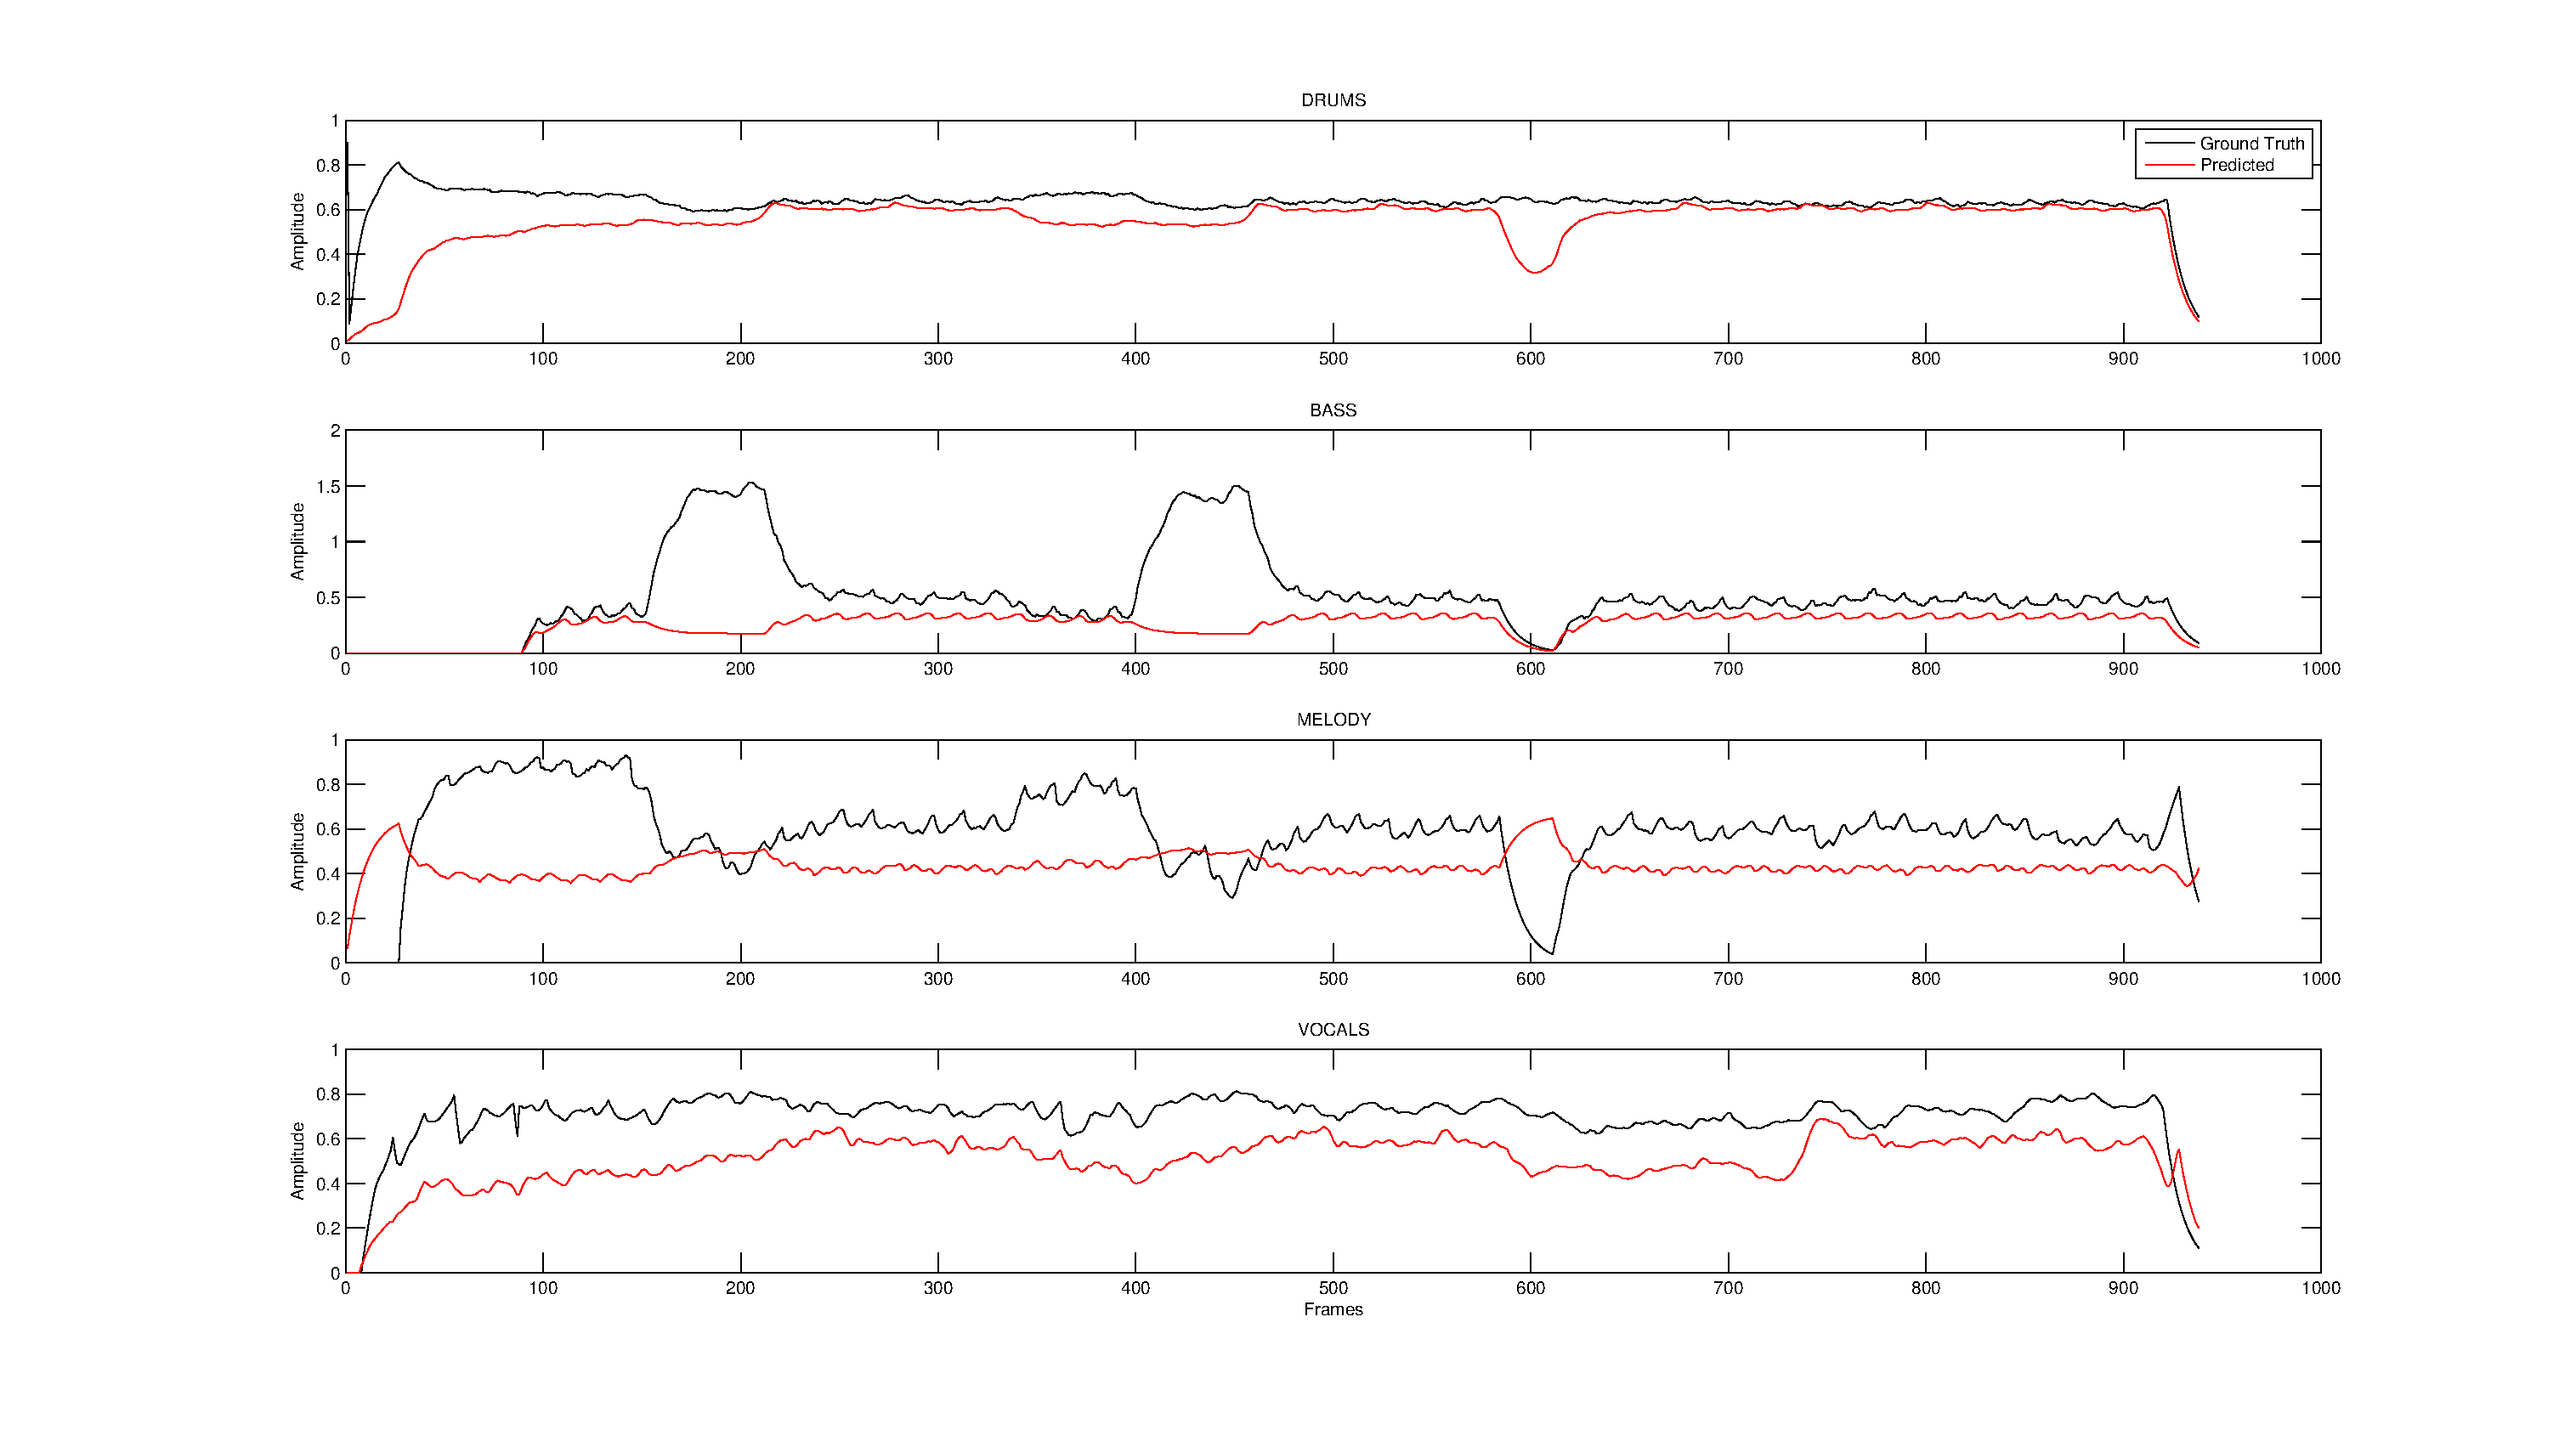
\includegraphics[height=200px, width=\columnwidth]{kp_cg.eps}%
\caption{Condition 1.}
\label{subfiga}%
\end{subfigure}%\hfill%
\begin{subfigure}{\columnwidth}
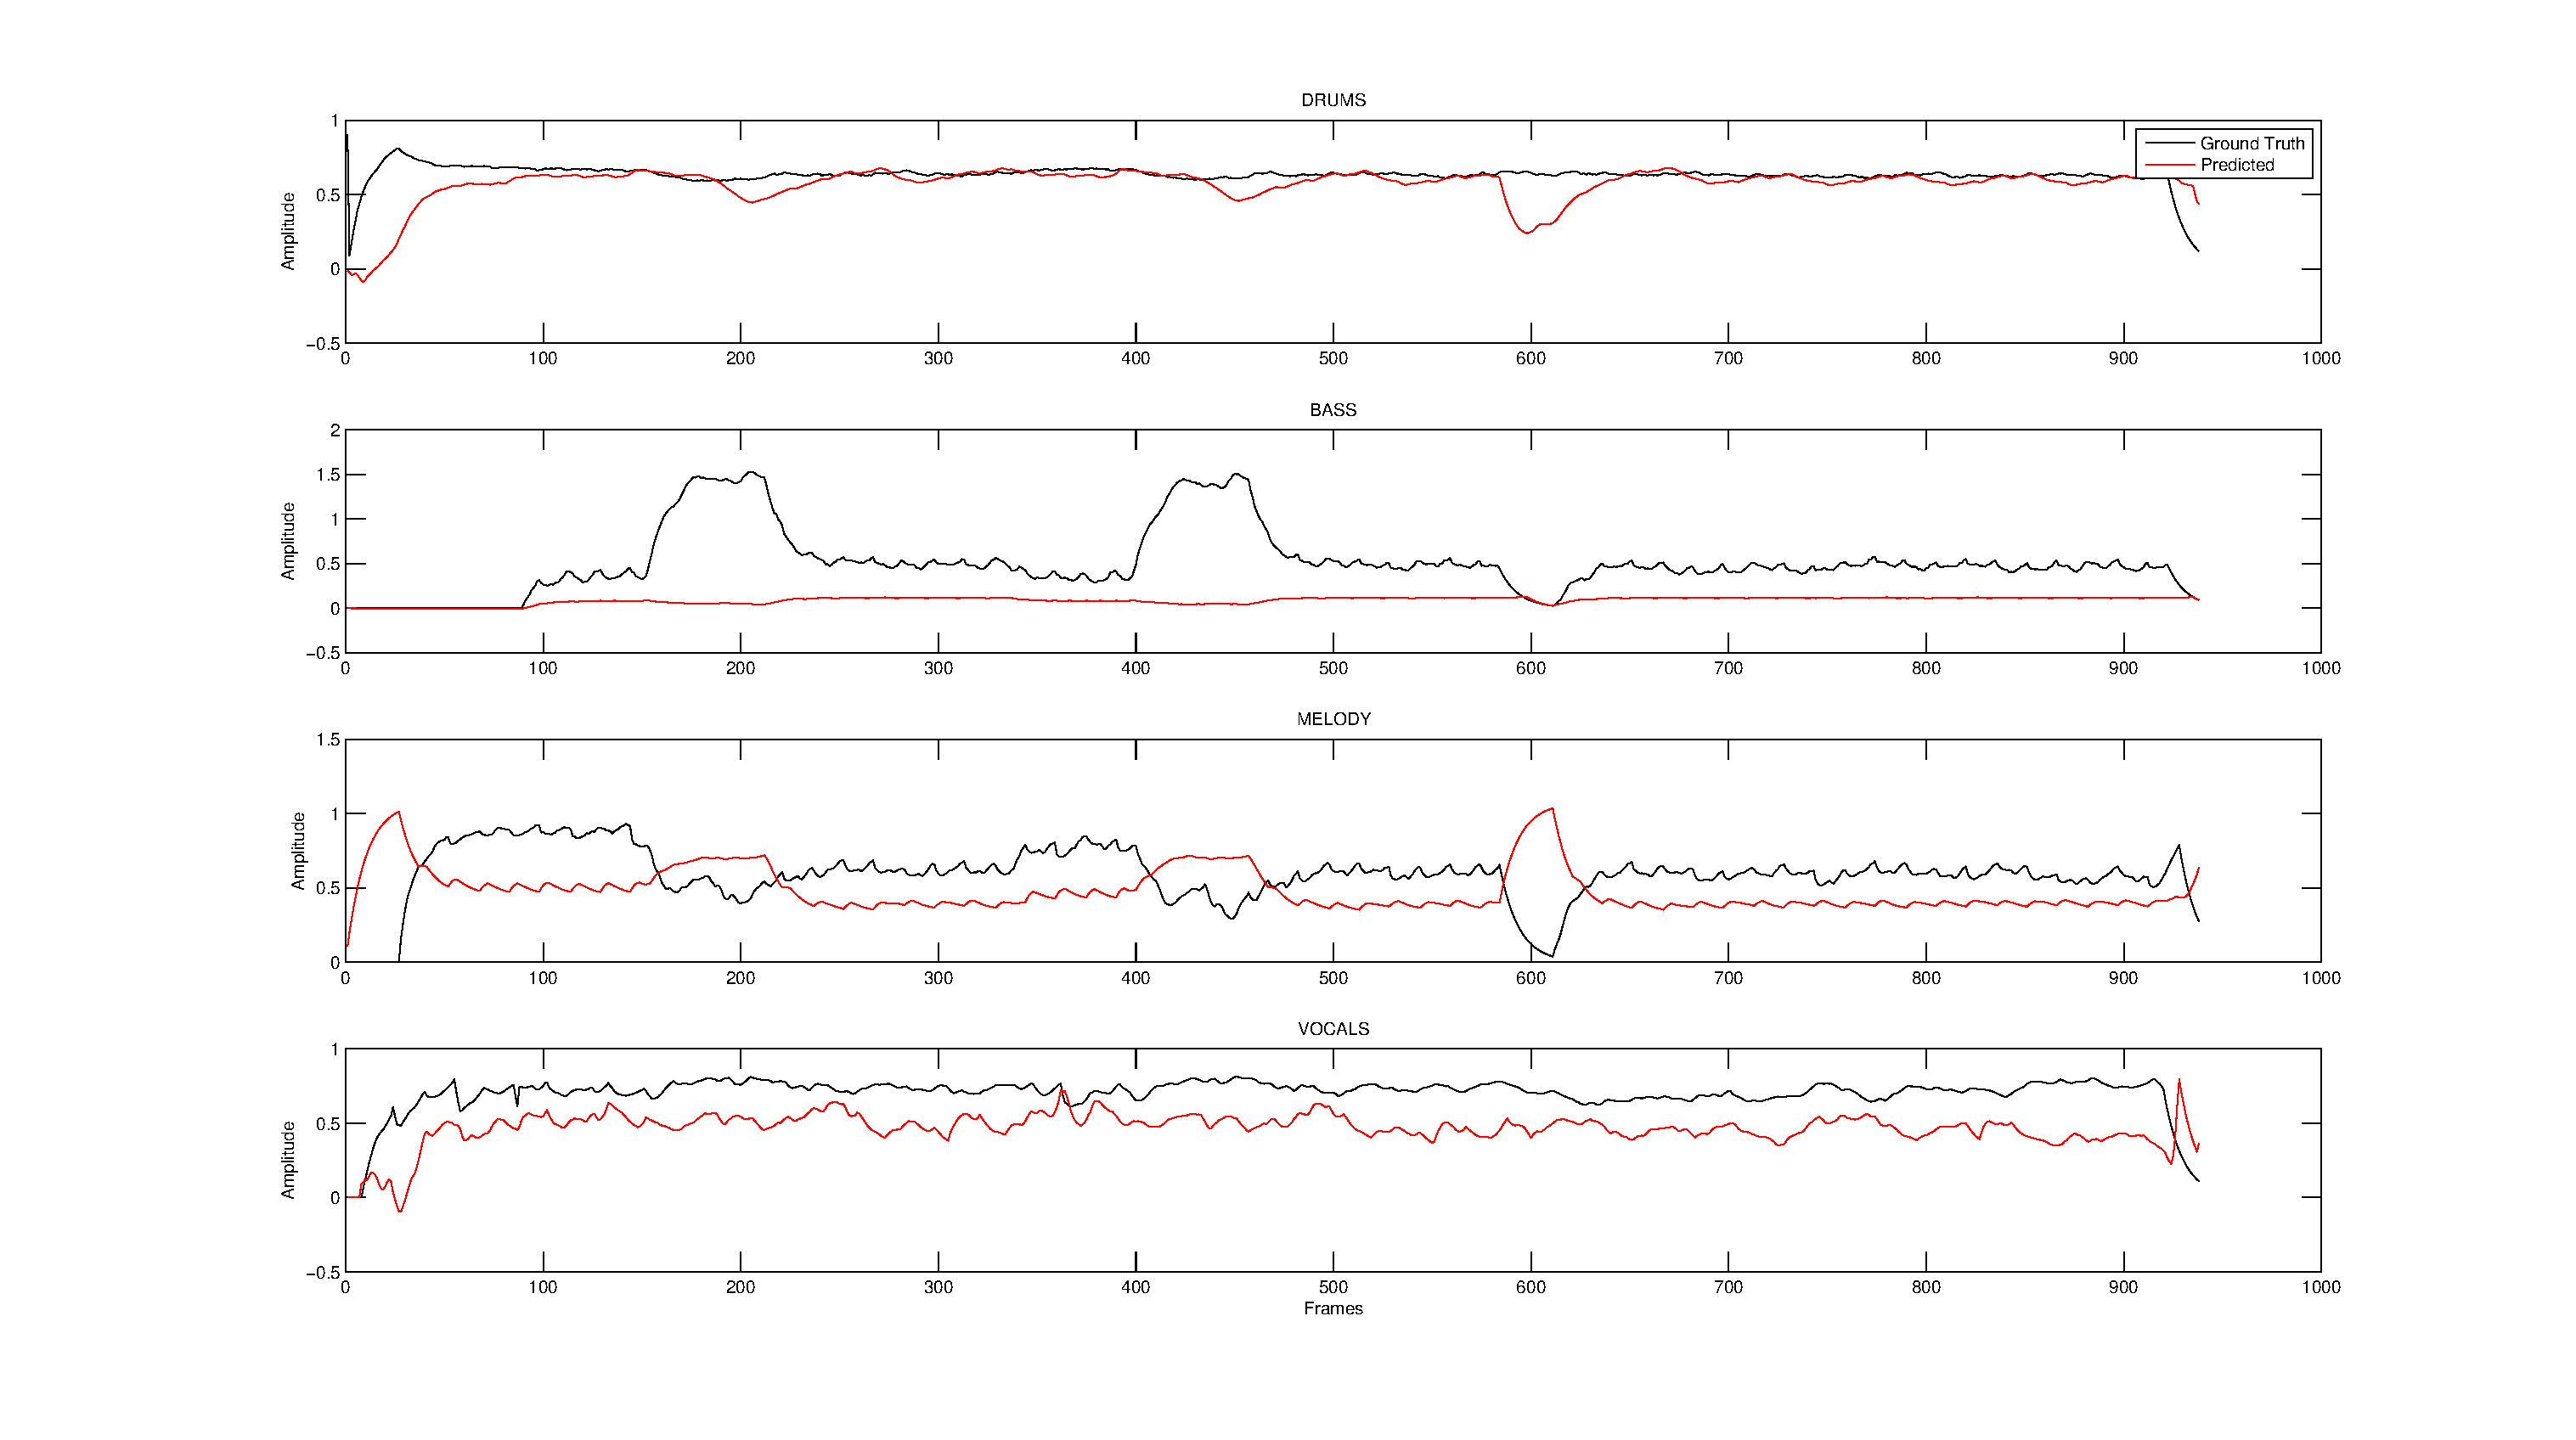
\includegraphics[height=200px, width=\columnwidth]{kp_cg_extrafeatures.eps}%
\caption{Condition 2.}
\label{subfigb}%
\end{subfigure}%\hfill%
\caption{Katy Perry - California Gurls, ground truth weights in black against predicted coefficients in red.}
\label{fig:katyperrycoef}
\end{figure*}

To attain the form given in equation \ref{eq:stftlinear}, the following process is executed.  First, for each track $k$ that contributes to the final mixture, the track is buffered into 1 second frames which overlap by 0.75 seconds.  This process is also executed for the master track $V$ so that at any time point $V_n$, $U_n\alpha \approx V_n$.  For each 1 second frame, a 1024 point STFT is computed with 50\% overlap.  The STFT for each track is then vectorized and concatenated such that the rows of $U(n, k)$ represent time while the columns represent each track $k$.  To improve the accuracy of the form given in equation \ref{eq:stftlinear}, if a track $k$ does not contribute to the final mixture at a given time point $n$, it is discarded.  To determine whether or not a track is active for a given frame, a simple thresholding is implemented such that if RMS$(k) < 0.01$, the track is considered inactive and not contributing to the final mixture.

Once we have attained our stem-matrix $U(n, k)$ and our final mix vector $V$, the ground-truth fader coefficients $\alpha_k$ can be extracted using non-negative least squares:

\begin{equation}
\hat{\alpha} = \min_{\alpha}||U\alpha - V||_{2}^{2}
\label{eq:NNNLS1}
\end{equation}

Due to the relatively short 1 second frame size, our ground truth coefficients are distractingly noisy.  In this implementation, a simple smoothing function is implemented via an exponential moving average filter to reflect a more realistic mixing coefficient:

\begin{equation}
\label{eq:EMA}
y[n] = (\alpha \cdot y(n-1)) + (1-\alpha) \cdot x(n)
\end{equation}

% FEATURE EXTRACTION
%----------------------------------------------------------------------------------------
\subsection{Feature Extraction}
\label{subsec:Feature Extraction}

In the original implementation of this algorithm referred to later in this paper as ``condition 1'', the following audio features were extracted to train the system:

\begin{itemize}
  \item Spectral Centroid
  \item RMS
  \item Spectral Slope
\end{itemize}

In the spirit of experimentation, we created a second condition (``condition 2'') with extra features to observe how they would effect the results.  These features were selected due to their relationship to the original features as timbral indicators and because they are unimodal.  The features used in this condition are:

\begin{itemize}
  \item Spectral Centroid
  \item The ITU-R BS.1770 Loudness Recommendation
  \item Spectral Slope
  \item Spectral Spread
  \item Zero Crossing Rate
\end{itemize}

\subsubsection{ITU-R BS.1770 Loudness Recommendation}
In addition to adding the spectral spread and zero crossing rate to our feature set, we opted to substitute an RMS calculation in favor of the ITU-R BS.1770 Loudness Recommendation as a more robust measure of a signals loudness.  In this loudness calculation, the signal is preemptively filtered to emulate the frequency response of the human ear before a subsequent modified RMS measurement.  The filter coefficients for a 48khz sampling rate are outlined in the original publication \cite{rec2006bs}, while a formula to calculate the coefficients for different sampling rates is given here \cite{mansbridge2012implementation}.  These filters can be easily implemented in MATLAB by supplying the proper filter coefficients to the \texttt{filt()} function. 

While the ITU-R BS.1770 standard was devised with mastered programmes in mind, autonomous mixing systems have been using it to quantify fader position coefficients.  Therefore, post K-filtering, the loudness for a given track $m$ is calculated by the following equation:

\begin{equation}
\label{eq:ITU-R BS.1770}
L_m[n] = 0.691 \cdot 10log_{10} \cdot \left(\frac{1}{N}\sum_{n=0}^{N-1}xg_m^2[n]\right)
\end{equation}

% MULTIPLE LINEAR REGRESSION
%----------------------------------------------------------------------------------------
\subsection{Multiple Linear Regression}
\label{subsec:Multiple Linear Regression}

At this point, we train our system to predict fader weighting coefficients based on the features extracted in section \ref{subsec:Feature Extraction}.  To train the system, we calculate the feature matrix $\bm{Y}(n, m)$ for every frame where $N$ is the number of frames in the song and $M$ is the number of features.  $\bm{Y}$ should be thought of as $\bm{Y}_k$, meaning we compute a feature matrix for each track in the song.  After we compute $\bm{Y}_k$ for each song in the training set, we then concatenate them together as $\bm{Y} _{train}$ to represent all the features collected for an instrument type across all songs.  We repeat the same process for $\alpha_{train}$ such that it becomes a matrix of weighting coefficients for all songs per instrument type.  With this data, we can compute a projection matrix $\hat_{\beta}$ using NNLS for any given instrument class $k$:

\begin{equation}
\hat{\beta} = \min_{\beta}||\bm{Y}\beta - \alpha||_{2}^{2}
\label{eq:NNNLS2}
\end{equation}

With our projection matrix, we can estimate the weighting coefficients for a given instrument in our test song with a simple matrix multiplication where $\hat_{\alpha}$ is our predicted coefficient for an instrument class $k$:

\begin{equation}
\[
\hat{\alpha} = \bm{Y}\hat{\beta}
\]
\label{eq:projectionmatrix}
\end{equation}

% AUTOMATIC MIX
%----------------------------------------------------------------------------------------
\subsection{Autonomously Mix}
\label{subsec:Autonomously Mix}

To create a new autonomously created mix down, we simply utilize equation \ref{eq:System Equation}, substituting $\alpha$ with $\hat_{\alpha}$ such that:

\begin{equation}
mix_t = \hat{\alpha}_{1t}u_{1t} + \hat{\alpha}_{2t}u_{2t} \dots \hat{\alpha}_{kt}u_{kt}
\label{eq:automix}
\end{equation}

%----------------------------------------------------------------------------------------
% RESULTS
%----------------------------------------------------------------------------------------
\section{Results}
\label{sec:Results}

To evaluate the performance of the system, a leave-one-out cross-validation method is used where training occurs on N-1 songs in the dataset and testing is performed on the remaining song.  An averaged mean squared error is then computed across all songs in the dataset.  The calculations described in section \ref{sec:Algorithm and Implementation} were calculated on two different data sets repeated by genre.  To experiment with the difference in coefficient calculation across genre, the training data from the rock dataset was projected onto a top-40 pop songs test data.  The difference between the spectral shape of the human mixed masters and the autonomous mixed masters is also compared.

% POP RESULTS
%----------------------------------------------------------------------------------------
\subsection{Top-40/Pop}
\label{sec:top40}

\begin{figure*}[!htbp]
\centering
\begin{subfigure}{\columnwidth}
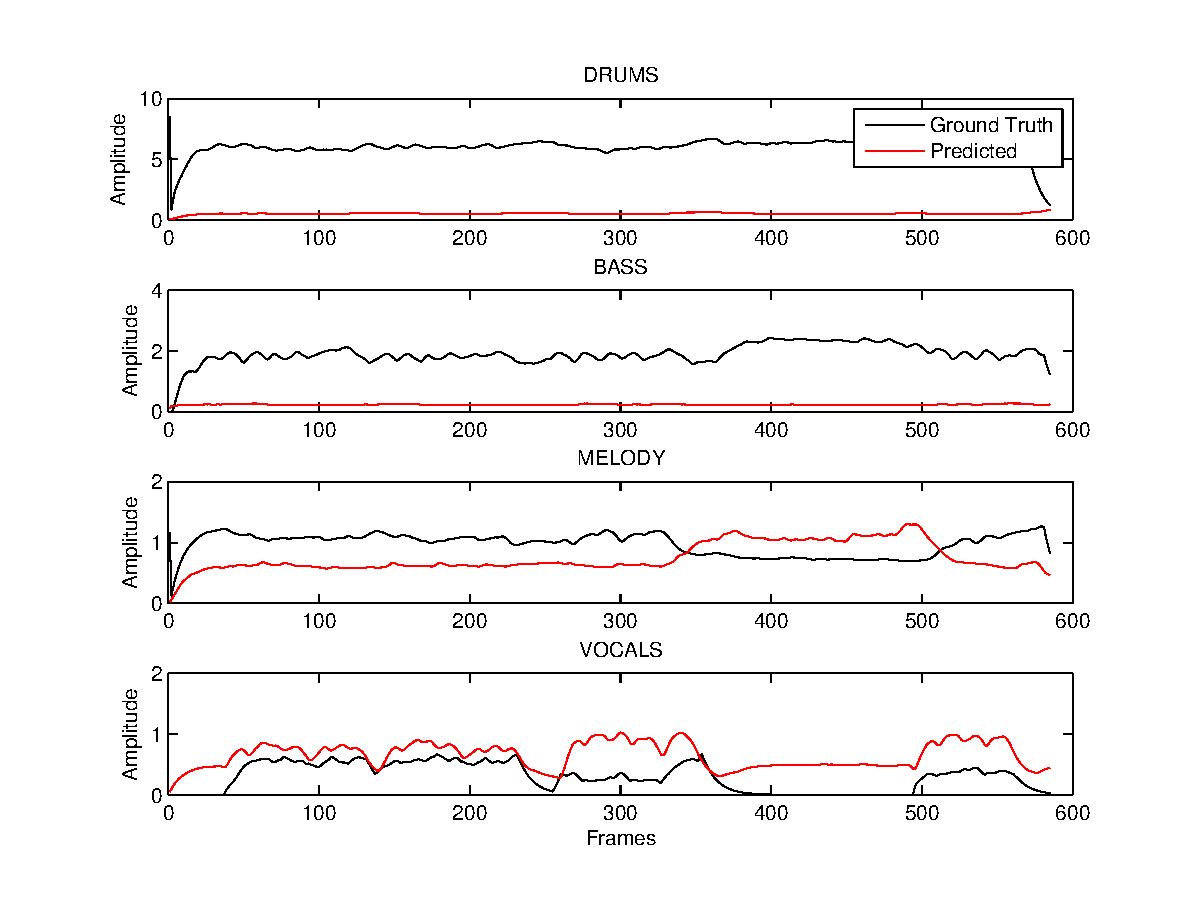
\includegraphics[height=200px, width=\columnwidth]{Plot_1_1.eps}%
\caption{Condition 1.}
\label{subfiga}%
\end{subfigure}%\hfill%
\begin{subfigure}{\columnwidth}
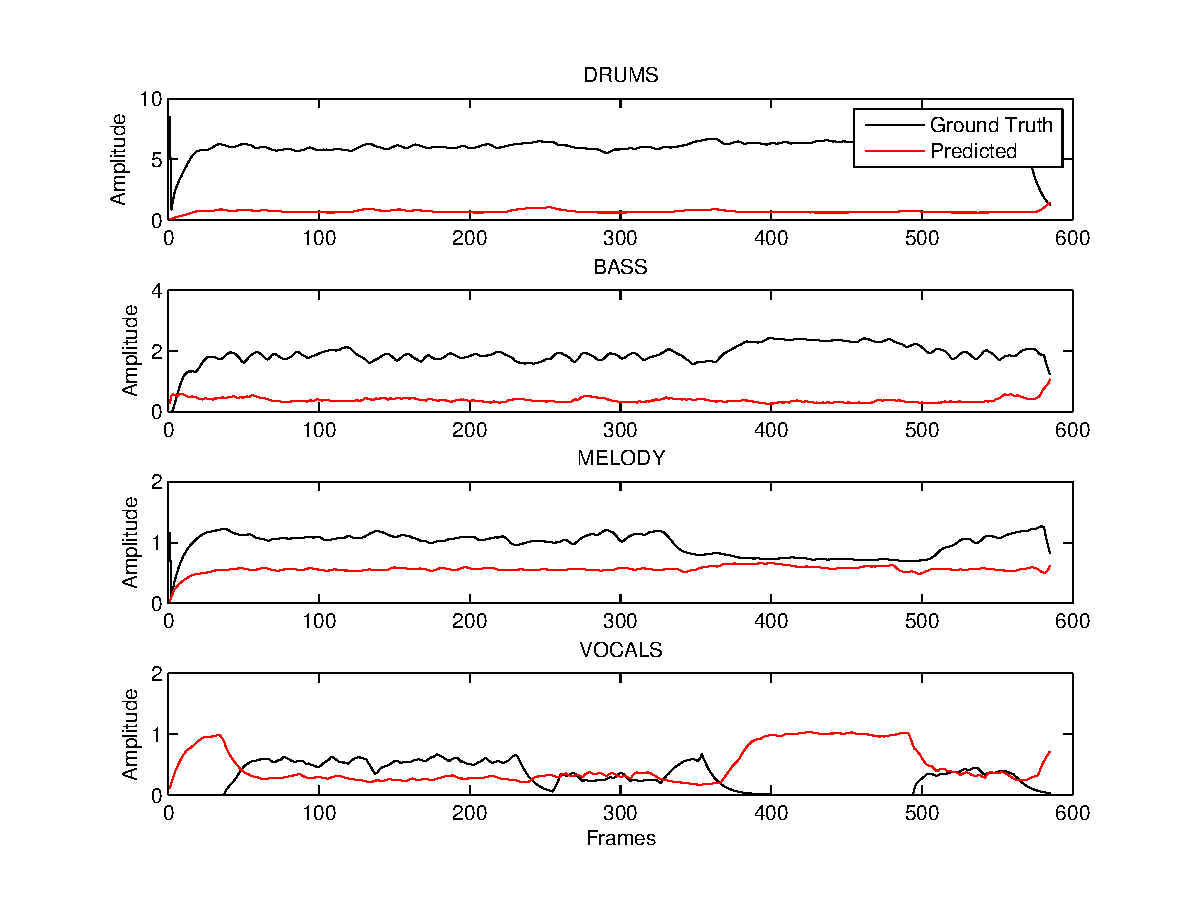
\includegraphics[height=200px, width=\columnwidth]{Plot_1.eps}%
\caption{Condition 2.}
\label{subfigb}%
\end{subfigure}%\hfill%
\caption{Big Troubles - Phantom, ground truth weights in black against predicted weights in red..}
\label{fig:bigtroubles}
\end{figure*}

Despite our small sample size of $(N = 7)$ for top-40 pop songs, the results are surprisingly good.  As we can see in figure \ref{fig:crossgenre}, our predicted coefficients for condition 1 are relatively accurate compared to the ground truths.  Unfortunately, we see a slight decrease in performance when evaluating under condition 2 which indicates that the new combination of features is less representative of weighting coefficients compared the original implementation.  Where table \ref{table:MSE-KP} shows the mean square error across one song, table \ref{table:MSE-pop} shows the averaged mean squared error across all songs and instruments under both test conditions.  Since the Fourier transform can be viewed as the linear combination of our weighted amplitudes in the frequency domain, we also plot the difference between the human engineered magnitude spectrum and the current automatically generated results in figure \ref{fig:difference_gaga}.

\begin{table}[h]
\centering
\begin{tabular}{ccc}
Track  & Condition 1 & Condition 2 \\ \hline
Drums  & 0.0204      & 0.0214      \\
Bass   & 0.1937      & 0.3118      \\
Melody & 0.0693      & 0.0924      \\
Vocals & 0.0438      & 0.0671      \\ \hline
\end{tabular}
\caption{Mean squared error comparing Katy Perry - California Girls ground truth weights against predicted coefficients.  Condition 2 adds extra features and substitutes LUFS instead of RMS.}
\label{table:MSE-KP}
\end{table}

\begin{table}[h]
\centering
\begin{tabular}{ccc}
Track  & Condition 1 & Condition 2 \\ \hline
Drums  & 0.0850      & 0.1648      \\
Bass   & 0.0174      & 0.1003      \\
Melody & 0.0775      & 0.1074      \\
Vocals & 0.1100      & 0.1126      \\ \hline
\end{tabular}
\caption{Mean squared error across all top-40 songs using leave-one-out cross-validation.  Condition 2 performs worse than condition 1 in predicting fader weighting coefficients.}
\label{table:MSE-pop}
\end{table}

\begin{figure}[h]
\begin{center}{\columnwidth}
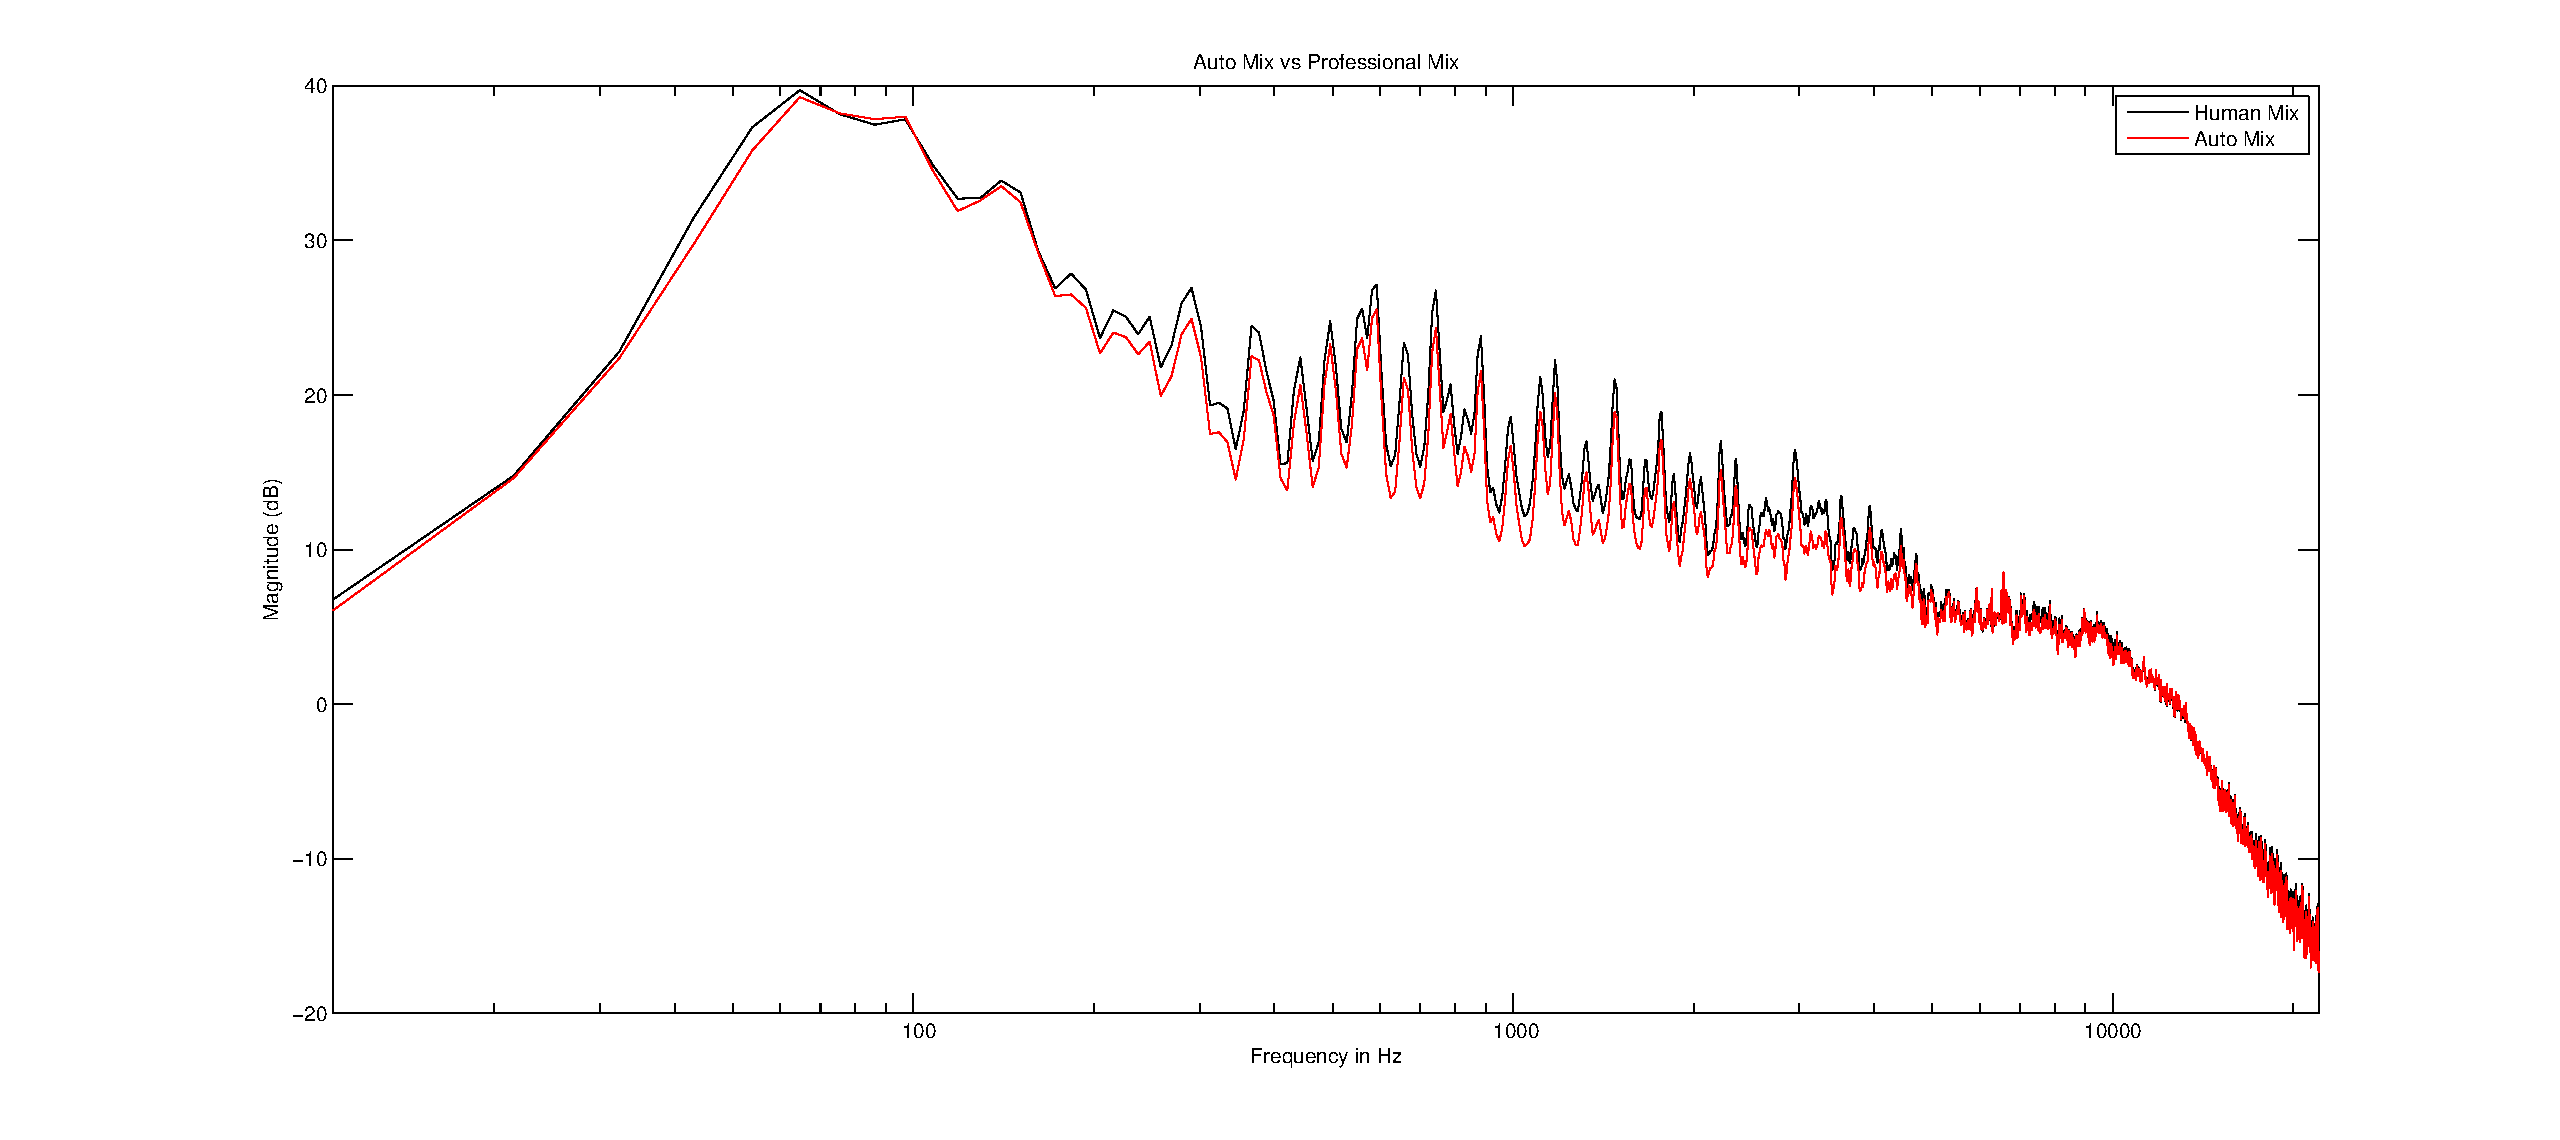
\includegraphics[height=100px, [width=0.9\columnwidth]{auto_mix_spectra-eps-converted-to.pdf}
\caption{Average magnitude spectra of human engineered and autonomously engineered mixes for Lady Gaga - Alejandro.  They are relatively similar, and the mean squared error corresponds to the differences in the frequency domain based on instrument.}
\label{fig:spectra_gaga}
\end{center}
\end{figure}

\begin{figure}[h]
\centering{\columnwidth}
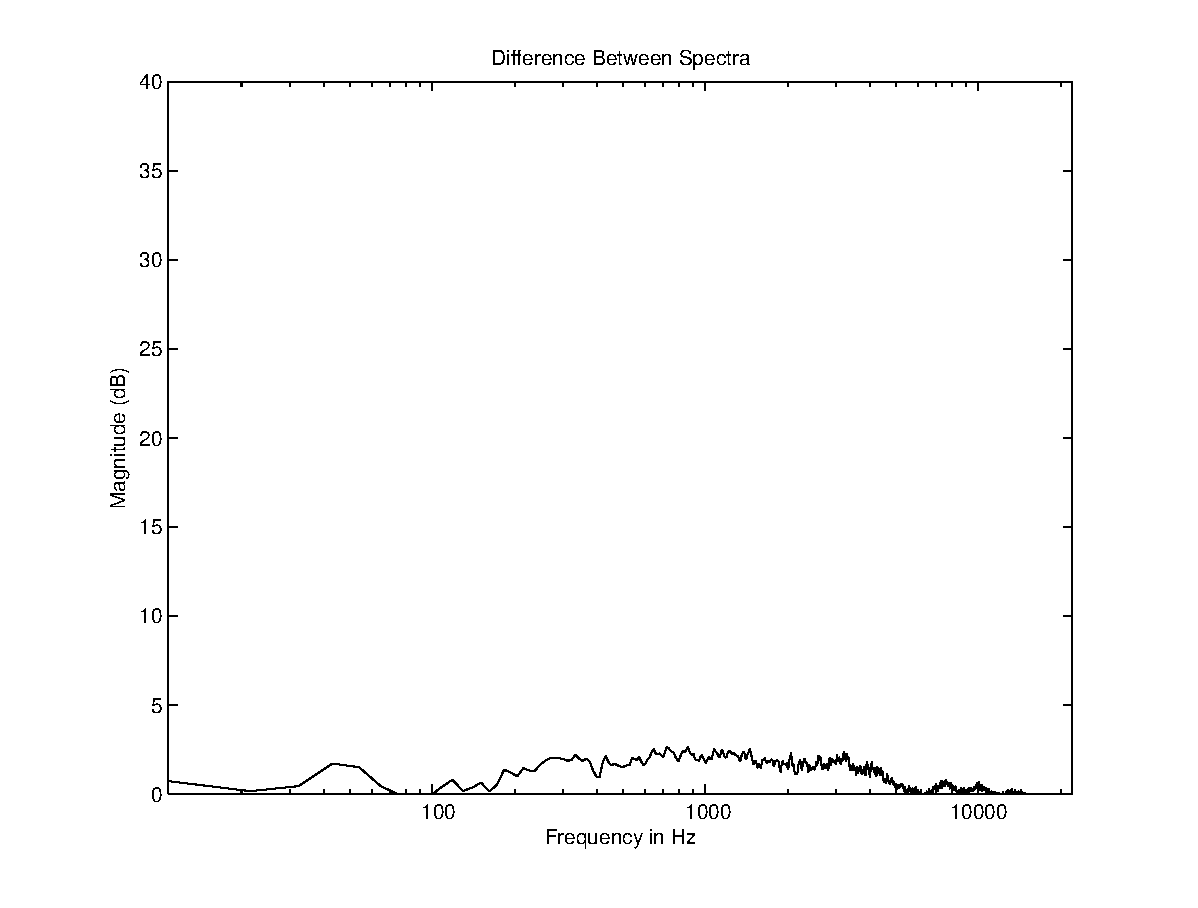
\includegraphics[height=150px, [width=\columnwidth]{lg_a_difference.eps}
\caption{The difference between ground truth $|X_{groundtruth}(\omega)|$ and $|X_{predicted}(\omega)|, $ $ \omega \in (0,\pi)$ .}
\label{fig:difference_gaga}
\end{figure}

% ROCK RESULTS
%----------------------------------------------------------------------------------------
\subsection{Rock}
\label{sec:rock}

When applying the aforementioned processing to the various rock tracks, it is clear that the algorithm is less successful through both the resultant autonomous mix as well as the mean square error.  As seen in figure \ref{fig:bigtroubles} significant discrepancies appear between the ground truth and predicted mixing coefficients.  This visual difference is supported by Table A where the MSE is shown for each track and particular observation can be made of the drum coefficients which produce astronomical MSE numbers.  Similarly, the difference in frequency spectra in figures \ref{fig:spectra_rock} and \ref{fig:difference_rock} shows how drastic this difference is, specifically in the lower frequencies below 300 Hz and the higher frequencies above 4 kHz.  The coefficients clearly mirror the pop results by producing a significant loss of lower frequencies, resulting in a mix that is noticeably heavy in the midrange.  

\begin{table}[h]
\centering
\begin{tabular}{ccc}
Track  & Condition 1 & Condition 2 \\ \hline
Drums  & 29.9624      & 28.1907      \\
Bass   & 2.8916       & 2.4489      \\
Melody & 0.1929       & 0.2087      \\
Vocals & 0.1602       & 0.2750      \\ \hline
\end{tabular}
\caption{Mean squared error comparing Big Troubles - Phantom ground truth weights with predicted coefficients.  Condition 2 adds extra features and substitutes LUFS for RMS.}
\label{table:MSE-rock1}
\end{table}

\begin{table}[h]
\centering
\begin{tabular}{ccc}
Track  & Condition 1 & Condition 2 \\ \hline
Drums  & 11.33758 \mp 16.85312      & 13.96146 \mp 16.00094     \\
Bass   & 2.08244 \mp 1.81634      & 2.03802 \mp 1.95372      \\
Melody & 0.30692 \mp 0.52348       & 0.24994 \mp 0.32676      \\
Vocals & 1.10308 \mp 2.74372       & 1.00838 \mp 2.93202      \\ \hline
\end{tabular}
\caption{Mean squared error across five rock songs using leave-one-out cross-validation.  Condition 2 performs similarly to Condition 1, with less accuracy for the drums but more accuracy for the melody.}
\label{table:MSE-rock2}
\end{table}

Although the results for mixes classified under the rock genre appear to be incredibly poor, analysis using leave-one-out cross-validation provides important insights into the nature of the error by utilizing various other test tracks.  Interestingly, the MSE during cross-validation changes drastically, as can be seen in Table B where the average MSE, as well as its range among test tracks, are shown using five different tracks for testing.  Clearly this difference provides a strong indication of the variety among songs used in the analysis, which speaks to the difficulties inherent in broad genre classification.

\begin{figure}[h]
\begin{center}{\columnwidth}
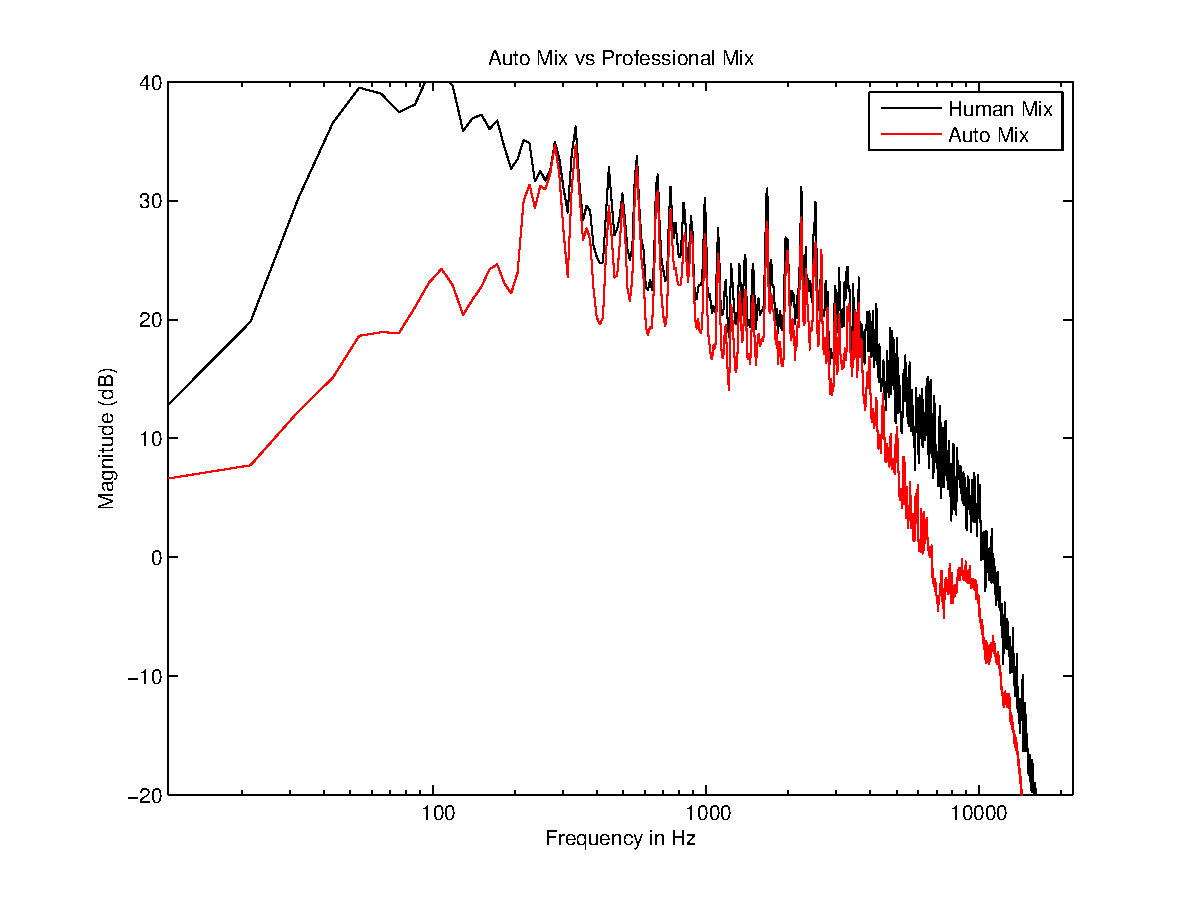
\includegraphics[height=150px, [width=0.9\columnwidth]{Plot_2_1.eps}
\caption{Magnitude spectra of human engineered and autonomously engineered mixes for Big Troubles - Phantom. They are noticeable dissimilar, and the mean squared error corresponds to the differences in the frequency domain based on instrument.}
\label{fig:spectra_rock}
\end{center}
\end{figure}

\begin{figure}[h]
\centering{\columnwidth}
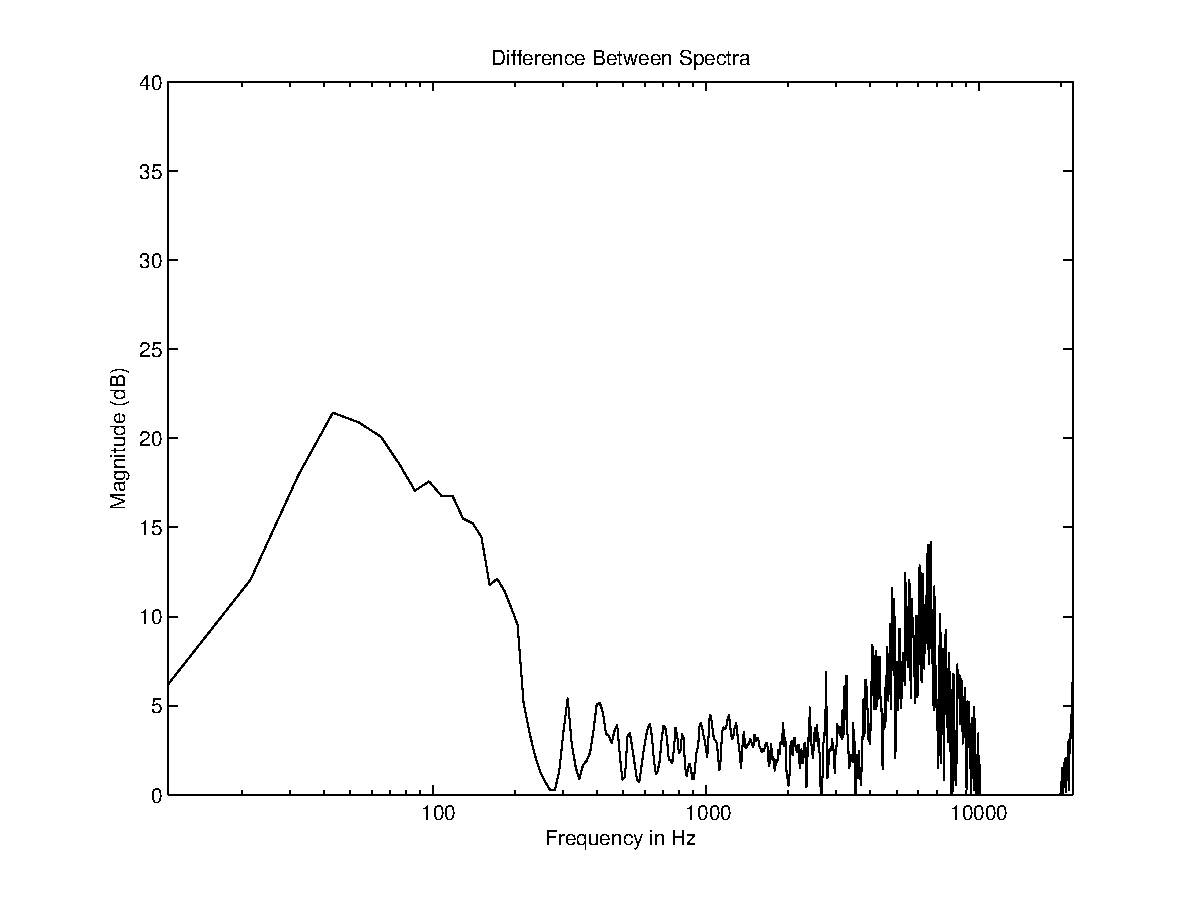
\includegraphics[height=150px, [width=\columnwidth]{Plot_3_1.eps}
\caption{The difference between ground truth $|X_{groundtruth}(\omega)|$ and $|X_{predicted}(\omega)|, $ $ \omega \in (0,\pi)$ .}
\label{fig:difference_rock}
\end{figure}

% CROSS-GENRE
%----------------------------------------------------------------------------------------
\subsection{Cross-Genre}
\label{sec:crossgenere}

For the following section, we experimented with applying weighting coefficients generated by the rock training data and applying them to a top-40 song to observe the difference in predicted coefficients between genre.  On paper the results don't appear to be that much worse than the original top-40 predictions, however subjective listening suggests that the mix generated via another genres coefficients is much less convincing than what was found in section \ref{sec:top40}.  As seen in section \ref{sec:rock}, the drums are especially under represented in the mix, these results are carried over to Britney Spears - Break The Ice where in table \ref{tabel:crossgenre} we see our largest error present in the drum track.

\begin{table}[h]
\centering
\begin{tabular}{ccc}
Track  & Cross Genre Test \\ \hline
Drums  & 0.1706           \\
Bass   & 0.0564           \\
Melody & 0.0267          \\
Vocals & 0.1337           \\ \hline
\end{tabular}
\caption{Mean squared error comparing Britney Spears - Break The Ice ground truth weights against predicted coefficients.  The training data here is from the rock genre dataset, creating some subjectively unpleasant results.}
\label{tabel:crossgenre}
\end{table}

\begin{figure*}[!htbp]
\centering
\begin{subfigure}{\columnwidth}
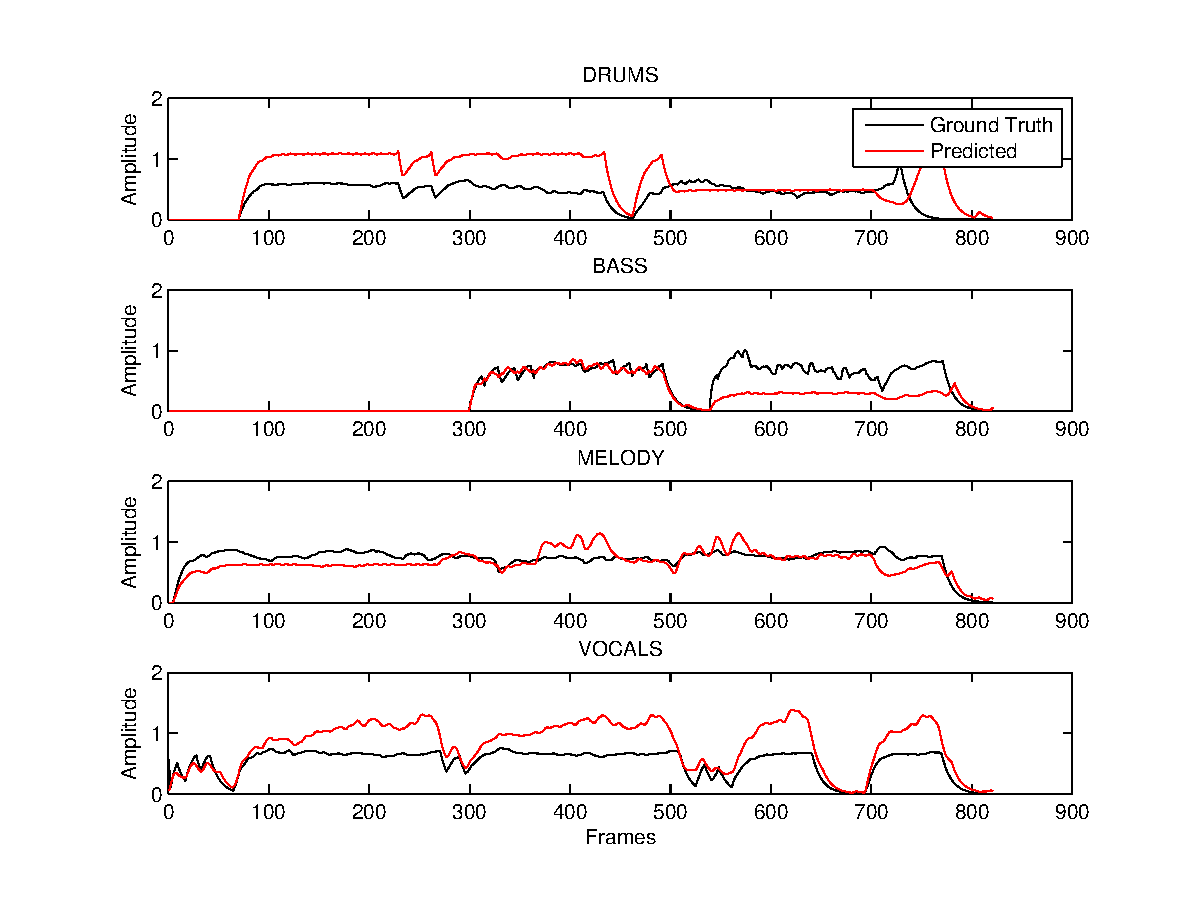
\includegraphics[height=200px, width=\columnwidth]{corssgenre1.eps}%
\caption{Condition 1.}
\label{subfiga}%
\end{subfigure}%\hfill%
\begin{subfigure}{\columnwidth}
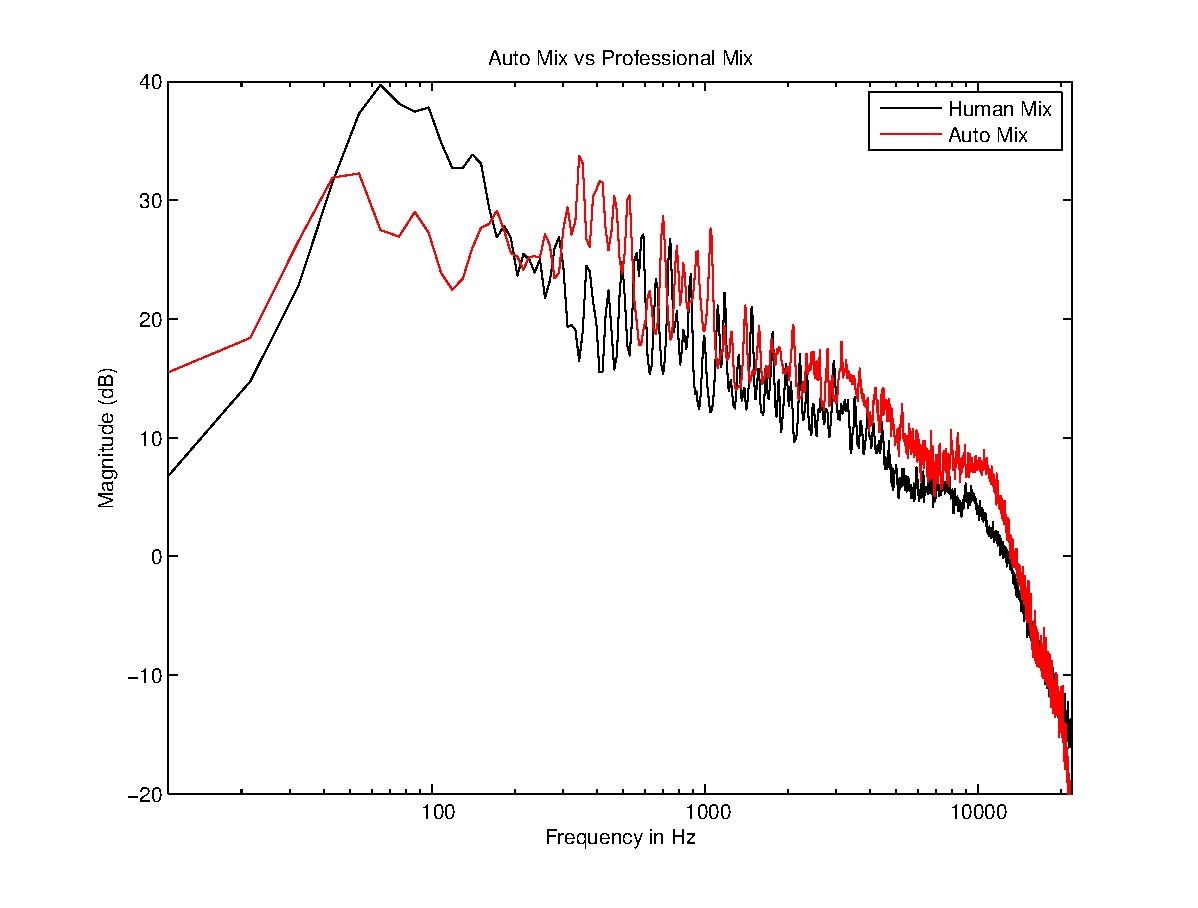
\includegraphics[height=200px, width=\columnwidth]{cross_genrespectra.eps}
\label{subfigb}%
\end{subfigure}%\hfill%
\caption{The spectra here is morphed from a typical top-40 spectra exhibiting a decrease in the low frequencies. This results in a much lighter sounding track with a flatter spectra, making the mix sound unbalanced as the upper frequencies mask the low frequencies.}
\label{fig:crossgenre}
\end{figure*}

%----------------------------------------------------------------------------------------
% Conclusion
%----------------------------------------------------------------------------------------
\section{Conclusion}
\label{sec:Conclusion}

The difference between the success of the algorithm for the pop genre versus the rock genre introduces an important consideration for this research.  Clearly the pop genre contained training and testing data from professionally recorded, homogeneous pop songs while the rock genre contained data from songs that were significantly less consistent.  For example, the training songs used could be classified as sub-genres ranging from shoe-gaze rock (Big Troubles - Phantom) to indie rock (The Districts - Vermont) and from punk rock (Meaxic - Take A Step) to classic rock (The Scarlet Brand - Les Fleurs Du Mal).  Because these subsets of the rock genre contain varying approaches to songwriting and track balance in particular, the comparatively poor predicted coefficients open the door for further analysis into the different artistic approaches to mixing among genres.  

Therefore, while a machine learning based autonomous mixing system was implemented successfully, its validity is weakened by the systems assumptions and limitations. While it is convenient to simplify the mix down into the summation of 4 separate channels, this does not represent how a mix is performed in reality.  One possibility for the future is to perform this same analysis in a recursive fashion such that this algorithm is applied to each of the 4 bus channels.  If this were to be implemented, we would then gain insight into the coefficients which sum to create the stems used in this experiment.  While this sounds good on paper, further inspection reveals that this process still requires the consolidating of data such that each bus contains the same number of elements and the same instrument classes.  Once again, this is not a valid assumption to make about a mix down as all songs have different instrumentation regardless of genre. 

Despite this, we attempted to improve the accuracy of this system by increasing the number of features which would characterize a stem and substitute the models calculation of loudness for a more modern widely accepted measure.  To our disappointment, objective evaluation shows that our version of feature extraction consistently performs worse than the previously implemented paradigm.  Oddly though, the authors find condition 2 to be subjectively more pleasing.  It's possible these subjective results can be attributed to the more stable coefficient values as seen in figure \ref{fig:katyperrycoef}, possibly giving off the perceptual quality of a more stable dynamic range between tracks.  Future research may want to experiment with expanding this model to incorporate the consideration of stereo field.  Unfortunately to the authors knowledge, there is no study which attempts to extract panning coefficients from professionally mixed data.  However, once the depth of this model is expanded, the methods in \cite{perez2010real} may be utilized to reduce masking between tracks which occupy the same fundamental frequency range.

One immediate source of data this research provides is genre and instrument specific weighting coefficients.  In the future, it would be immensely useful to test whether or not a system can identify a genre and instrument class based upon ground truth weighting coefficients.  At the very least, an analysis can be conducted which attempts to find patterns between these measures, helping mix engineers in the future make knowledge informed decisions, or incorporating this data into a knowledge engineered cross adaptive system such as in \cite{de2013knowledge} or \cite{scott2013instrument}.

The state of the music industry is one where anyone with a laptop and an idea can create a song.  Excluding the valid reasons outlined in section \ref{sec:Introduction} for pursuing this research, a huge market is waiting for this technology to exist.  Autonomous mastering has already made it to market in the form of Landr (https://www.landr.com/), created and engineered by many of the leading researchers referenced in this paper.  The authors believe that the data and methods presented here are convincing enough to pursue further, and looks forward to future developments in the field.

%----------------------------------------------------------------------------------------
% Bibliography
%----------------------------------------------------------------------------------------
\bibliography{Zafrin_Chudwick_MIRFP}

\end{document}
